\chapter{Background}
\label{ch:background}

\section{Solar water heating systems}

\subsection{Need and uses}

As we enter the twenty-first century, sustainability, energy security, and new ways to meet our increasing energy demands are on the agendas of many governments.
In Australia, water heating is the second-largest residential energy end use, accounting for an estimated 23\% of energy consumption, according to the Commonwealth government's Residential End-Use Monitoring Program~\cite{REMP12}.
This is second only to HVAC (air conditioning and space heating).
In some nations, the number may be as high as 30\% to 50\%~\cite{Lane96}.
Therefore, using `free' solar energy to heat water is an obvious way to significantly reduce domestic power consumption.

Two approaches are immediately obvious when considering heating water by catching sunlight: direct heating, which is the subject of this thesis, and using photovoltaics to heat water with electricity generated from the sun.
Though this thesis simulates a direct water heating system, since both types involve a heated water tank the resulting controller is likely to be easily adapted to photovoltaic systems as well.

\subsection{Economics}

\textcite{Fitzmorris10} performed an economic analysis of the current SDHW industry in North America.
He found that although solar water heating is positioned to be a disruptive technology, due to its superior energy efficiency compared to traditional water heating, it was actually losing market share due to problems in supply chain and the increased up-front cost of these systems.
He identified two important markets: construction firms who want to minimise the cost of a new house, and homeowners who need to replace a broken heating system.
The former is sensitive to the highly increased price of the solar system (Fitzmorris estimates up to \$2000 for a solar system installation, versus \$300 for an electric heater).
The latter market is sensitive to the increased complexity of installing a solar system --- there is more design work involved in properly sizing and installing a solar water heater currently, and replacement speed is typically a deciding factor.

Once a solar water heating system is running, though, the gains are found to be significant.
Anecdotally, the University of Newcastle reported a nearly-80\% reduction in energy use (and energy bill) in a six-storey teaching and research building~\cite{ApricusNewcastle}.
Less anecdotally, members of the School of Energy and Power Engineering at the Xi'an Jiaotong University designed and studied a SHWS for a hotel in the city~\cite{Cao14}.
They considered a replacement for the hotel's current gas geyser water heater, and predicted that it would have a payback period of just 7.4 years, as well as a lower \emph{total} investment over its 20 year lifetime than the \emph{initial} amount spent on the gas geyser heater.
This analysis included the benefits of carbon credits the hotel would receive from the government.

However, this feasibility is obviously location-dependent.
\textcite{Greening14} concluded that ``the potential of solar thermal systems to contribute to a more sustainable domestic energy supply in the UK is limited'' due to their poor effectiveness in that nation's climate.
He also identified the reliance on a backup heating system as a significant weakness and disadvantage when compared to other heating systems.

\subsection{System overview}
\label{sec:background:system}

Solar domestic hot water systems refer to services that use solar energy to heat hot water for domestic uses.
This involves a large collector panel attached somewhere it will receive direct sunlight, usually on a roof or awning.
The solar collector receives cooler water from the user's existing hot water tank, which is pumped slowly through the collector, being heated by the sun as it goes.
This hotter water is then pumped back into the hot water tank.
\Autoref{fig:hot-water-service} illustrates this.

\begin{figure}
   \centering
   \includegraphics[width=10cm]{images/house}
   \caption{Overview of a typical domestic water service}
   \label{fig:hot-water-service}
\end{figure}

These systems have a number of variables in their design.
The following list will highlight some of the most important factors, and most relevant to this thesis.

\begin{description}
   \item[Water loop] An open-loop system is one in which the water circulating through the collectors is potable and is passed directly to the load.
      In a closed-loop system, by contrast, the collector has its own circuit and liquid is not passed from it to the user.
      This means that, for example, anti-freeze chemicals can be added to the collector loop.
      In this case, a heat exchanger must be used to transfer heat from the collector loop to the storage tank.

   \item[Flow control] Some systems include a bypass that allows water from the collector output to bypass the storage tank and be returned to the collector input for further heating.
      This means that water does not have to enter the tank until it is warm enough, but water can be kept moving through the collector to avoid stagnation.
      Most systems also include safety release valves on either the tank or collector (or both), allowing excess pressure and heat to be released on hot days.

   \item[Hydronics] Applications are not limited to providing potable hot water for taps.
      Hydronic systems use hot water for space heating, often on a separate loop to potable water.
      This may be achieved using radiators, or by passing the water through pipes in floors.

   \item[Scale] Solar hot water services must obviously come in many sizes to fulfil the requirements of different users.
      The variables include the size of the water tank itself, the area of --- and water volume in --- the solar collectors, and the power of the auxiliary booster.
      Solar systems are typically sized for a specific user's summer consumption requirements, to avoid overheating, though this means their performance in winter is low.
\end{description}

\subsection{Control}

Current hot water systems typically use simple temperature-differential controllers to force water through the solar collectors and to decide when to use a secondary booster to heat the tank water.
This approach is outlined in Sustainability Victoria's handbook for solar thermal system design~\cite{LSTS}.
The handbook points out that simple controllers such as timers or single sensors cannot adequately react to the entire system state --- for example, variations in insolation across a day, or variations in the storage temperature of the tank.
For this reason, it recommends the use of temperature differential controllers.

Simply, the temperature of the water exiting the solar collectors is compared to the temperature in the tank, and the pump is activated if there is a positive difference (i.e.\ useful heat is available).
The handbook goes on to detail refinements to this approach --- using proportional motor speeds instead of binary control, hysterisis to avoid pump hunting (rapid on/off motor cycles), and also mentions integration with building automation systems and ``time-of-day clocks \ldots for applications that have a repeated daily hot water demand pattern.''

Additional insight is provided in a 1994 paper by~\textcite{Beckman94} in which the process of designing these binary differential controllers is analysed.
They primarily cocern themselves with designing hysterisis bands that result in stable simulations, in order that fair and correct results may be obtained when comparing system ratings.
They note that in practise, this instability in pump control is rarely a problem because ``solar radiation is generally increasing continuously (in the morning) and the system soon reaches a stable condition''.

\subsubsection{Stratification}
\label{sec:background:stratification}

The heart of the domestic hot water service is the tank where hot water is stored waiting for the user to demand it.
(While tankless systems may provide efficiency gains~\cite{DuffBradnum13}, they are unable to store solar heat and use it when the sun is not shining, and therefore forgo most of the free energy the sun provides.)
Tank stratification is an important concept to understand and account for when considering these systems.

Stratification is the natural tendency of water to form layers of uniform temperature, between which there is relatively little heat flow.
\textcite{Hollands89} review the benefits of maintaining stratification in a hot water storage tank in their 1989 paper.
At this point, stratified tanks were just beginning to become the preferred paradigm for storage in domestic hot water systems.
Their review points out that systems that maintain tank stratification (usually by designing for low flow rates, but potentially by using good diffusers inside the tank) can improve performance by nearly 40\% in some circumstances.
This is an effect of lower-temperature water entering the solar collector.

These diffusers have been investigated in studies such as \textcite{Andersen08} and \textcite{Gari82}.
While they may still not be common in commercial hot water systems, diffusers appear to be a proven technology.
A diffuser typically takes the form of a pipe running the length of the tank, either of slotted platic or double-layered fabric.
Water is inlet into the pipe, and it allowed to travel vertically before it naturally diffuses out of the manifold at a height matching its temperature.
In this way turbulent mixing is mostly localised to within the manifold, and overall tank stratification is preserved.
The mathematical model used and extended by this thesis relies on the presence and operation of these stratification-enhancing devices.

\section{Model-predictive control}

\subsection{Overview and comparison to PID control}

As described by \textcite{Camacho04} in their work on the subject, model-predictive control (MPC) is a class of control strategies that incporate an explicit model of the system into their decision-making process.
Note that this model may include the system's input response, disturbance response, predictions of time-varying effects, etcetera.
The typical implementation of MPC follows this simplified flow:

\begin{enumerate}
   \item Measure or estimate current state and predict disturbances.
   \item Optimise sequence of control inputs over some finite time horizon.
   \item Apply the first input to the system.
   \item Repeat at next time interval.
\end{enumerate}

Note that although a plan of inputs is generated over a time horizon, the entire plan is not usually used.
This strategy has a natural analogy in pathfinding; it is necessary to plan the entire path to determine which direction to move in first.
However, as the system model and disturbances are usually not perfectly known, the system will diverge somewhat between iterations of the algorithm, and therefore the remainder of the input sequence may be invalidated.
In this way, feedback control is achieved by repeatedly responding to the current system state.

\authors{Camacho04} compare MPC to PID by likening PID to driving a car by only looking in the rear-view mirror.
In this situation, the driver can only respond to past errors, as PID does --- achieving pure feedback control.
MPC allows future conditions to be anticipated and explicitly included in the decision-making process.
MPC is not an optimal control technique like the LQR, but at every control instant (item 2 in the algorithm description above) a finite-horizon optimal control problem is solved.

Note that some techniques may allow PID to emulate the output of MPC on some systems.
For example, where a reference signal must be tracked, and the signal has a known schedule, the signal may be transformed forwards in time so that the PID controller starts responding earlier.
However, MPC will determine the best course of action itself without requiring manual intervention.

\subsection{Application to hot water services}

This author believes that model-predictive control is a strong fit for control of hot water services.
Firstly, the system is underactuated and heavily affected by disturbances.
These disturbances \emph{can}, however, be predicted and planned for, at least in the short term (matters of hours).
The Nest thermostat has shown that it is feasible to predict user activity, and use this to optimise building control.

Further, domestic systems may involve interaction with the user --- thermostats that control home air conditioning are an example, as are the `eco modes' becoming more common in automotive control systems.
MPC affords the possibility of easily designing and specifying tuning parameters that a user can interact with, due to its declarative and intuitive nature.
This will be seen in later sections.

\subsection{Linear systems}

Model-predictive controllers solve an optimisation problem at every instant in time to determine the next control input.
When controlling a system whose dynamics can be modeled linearly, the form of this optimisation problem is, in general,
\begin{equation}
   \label{eq:mpc-opt}
   \begin{aligned}
      & \underset{\vec{u}}{\text{minimise}}
      & & f^*(\hvec{y}, \vec{u}) \\
      & \text{subject to}
      & & \hvec{y} = \Psi \vec{x}_0 + \Theta \vec{u}, \\
      &&& f_i(\hvec{y}, \hvec{u}) \le 0\ \text{for all $i$}, \\
      &&& g_j(\hvec{y}, \hvec{u})   = 0\ \text{for all $j$}. \\
   \end{aligned}
\end{equation}
The controller attempts to minimise the chosen objective function $f^*$ while satisfying the system dynamic constraints.
$\Phi$ and $\Theta$ encode these linear dynamic constraints on the output $\hvec{y}$ given the input $\hvec{u}$, over some time horizon usually referred to as $H$.
More detail on this problem formulation is found in \autoref{sec:models:control}.

Note that the general constraints in this problem, $f_i$ and $g_j$, are representative of meaningful constraints in the context of a particular problem.
They are given here in generic form to denote that there may be constraints in the form of both equlities and inequalities.
The constraint on system dynamics is one of these equality constraints, which has been singled out for its particular universality in linear MPC problems.

\section{Convex optimisation}
\label{sec:background:convex}

\subsection{Mathematical background and significance}

Convex optimisation refers to the class of mathematical optimisation problems where the objective and constraint functions are all convex with respect to the decision variable(s)~\cite{Boyd04}.
Convexity, briefly, is the property that a function is `bowl-shaped'.
It must at all points obey Jensen's inequality:
\begin{equation}
   \label{eq:jensen}
   f(\theta x + (1-\theta)y) \le \theta f(x) + (1-\theta) f(y).
\end{equation}
That is, in between any two points, the function must lie on or below the direct line between those points.
\Autoref{fig:convexity} illustrates this property.
Importantly, this implies that any local minimum of the function will also be a \emph{global} minimum.
This property means that gradient descent algorithms can be guaranteed to find the global optimum of the function, and very efficient solvers can take advantage of this.

\begin{figure}
   \centering
   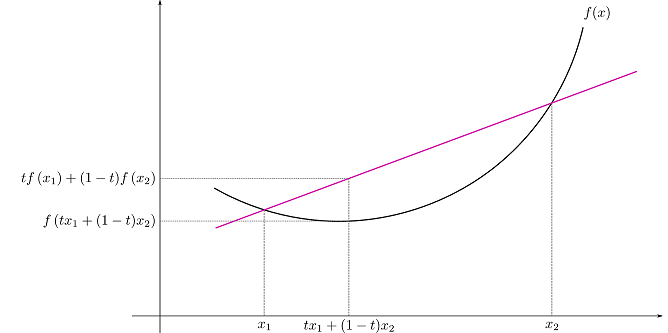
\includegraphics[width=10cm]{images/convexity}
   \caption{An illustration of Jensen's inequality from \autoref{eq:jensen}}
   \label{fig:convexity}
\end{figure}

Since the core of model-predictive control algorithms involves optimising the choice of cost function over the future control sequence, convex optimisation problems play an important role in its implementation.
Note that if a system is linear and its objective function and constraints are convex, the optimisation problem governing its control can be convex, and hence efficiently solved.

\subsection{Disciplined convex programming}

While the theoretical advantages of using convex optimisation are widely known~\cite{Luo06}, in practise these rewards may be difficult to reap.
While there exist general-purpose solvers for non-smooth convex optimisation problems which have attractive theoretical properties, they may in practise be slower than transforming a non-smooth problem into a smooth problem of higher dimension, and using an efficient solver for the new problem class.
Grant and Boyd opine that this process is difficult and error-prone, even for experts in the field~\cite{Grant08}.
They propose a method called \emph{disciplined convex programming} (DCP)~\cite{Grant06} which aims to express convex optimisation problems in such a way that transformation to an efficiently-solvable representation can be automated, removing this ``expertise barrier'', as they put it.

Recent DCP software such as CVX for MATLAB~\cite{CVX} and CVXPY in Python~\cite{CVXPY} implements this paradigm to provide a simple user interface without sacrificing the efficiency of specialised solvers for subclasses of convex problems.
